% !TEX root = ../main.tex
\section{FMT Alignment and Reconstruction}
\label{12::fmt_alignment_and_reconstruction}
    In paper, the FMT offers a 3 to 10-fold increase in resolution when compared to DC \cite{aune2009}.
    Achieving this improvement requires work on the alignment and calibration of the detector, as well as the reconstruction from its data.
    This chapter focuses on the work carried out in this endeavour, specifically addressing alignment and reconstruction.

    The first section provides a detailed description of Micromegas detectors in general and the FMT in particular.
    Subsequently, the second and third sections discuss the efforts made in alignment and reconstruction, respectively.
    Finally, the fourth and final section of the chapter elaborates on the resolution improvement resulting from this work.

    % !TEX root = ../main.tex
\subsection{Forwards MicroMegas Tracker}
\label{12.10::forwards_micromegas_tracker}
% --+ Micromegas +--------------------------------------------------------------
    \begin{figure}[b!]
        \centering\frame{
        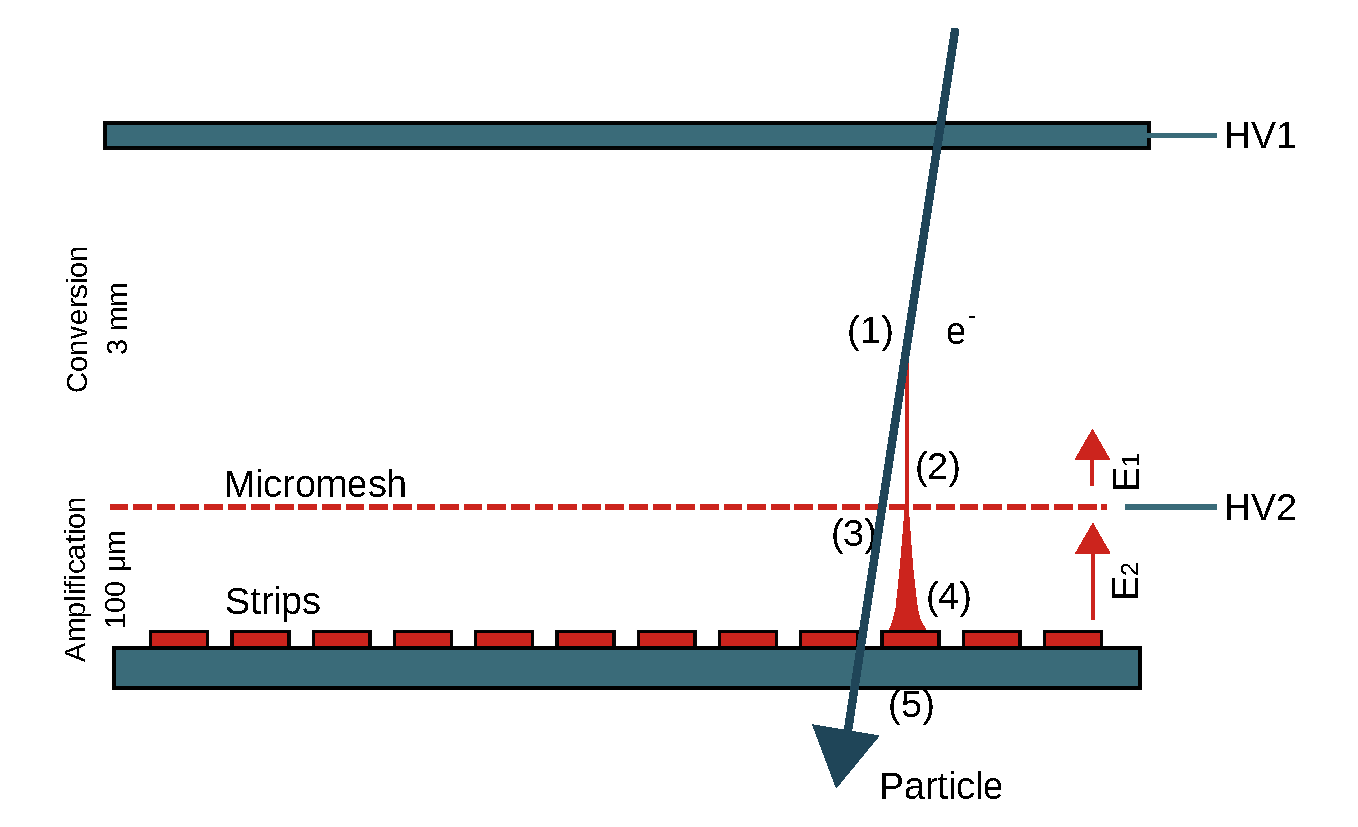
\includegraphics[width=\textwidth]{10mm_principle.pdf}}
        \caption[MM working principle.]{MicroMegas working principle.
        Source: Re-render of original illustration by \cite{giomataris1996}.}
        \label{fig::12.10::micromegas_principle}
    \end{figure}

    A Micro-Mesh Gaseous Detector or MicroMegas (MM) is a gaseous particle detector that is derived from wire chambers.
    These types of detectors are commonly used in experimental physics for detecting ionising particles.
    The MM detector offers very precise temporal and spatial resolution, on the order of 100 nanoseconds and below 100 micrometers \cite{giomataris1996}.

    The detector operates by amplifying the charges created by ionisation in the gas volume.
    Its volume is divided into two parts by a metallic micro-mesh placed less than 150 micrometers away from the readout electrode or strip.

    To illustrate this process, refer to Figure \ref{fig::12.10::micromegas_principle}.

    When a particle passes through the detector, it ionises the gas atoms by stripping an electron, resulting in an electron-ion pair (1).
    An electric field, denoted as $\text{E}_1$, is applied to the gas, causing the electron to drift towards the amplification electrode (2) while the ion moves towards the cathode.
    As the electron crosses the mesh (3), it enters a strong electric field, denoted as $\text{E}_2$, triggering an avalanche effect (4).
    This produces a significant signal at the readout strip (5), which can then be stored for reconstruction \cite{giomataris1996}.

% --+ Micromegas in CLAS12 +----------------------------------------------------
    Inside the CLAS12 detector, a diverse set of tracking detectors is utilised to determine the positions and momenta of particles at different points along their trajectories.
    The proximity of these detectors to the particle source directly correlates to the precision achieved in determining the position and momentum at the interaction vertex, which refers to the point where the particle was generated.
    To optimise this precision, the MicroMegas Vertex Tracker (MVT) in CLAS12 is positioned as close as feasible to the target, as depicted in Figure \ref{fig::12.10::micromegas_vertex_tracker}.

    \begin{figure}[b!]
        \centering\frame{
        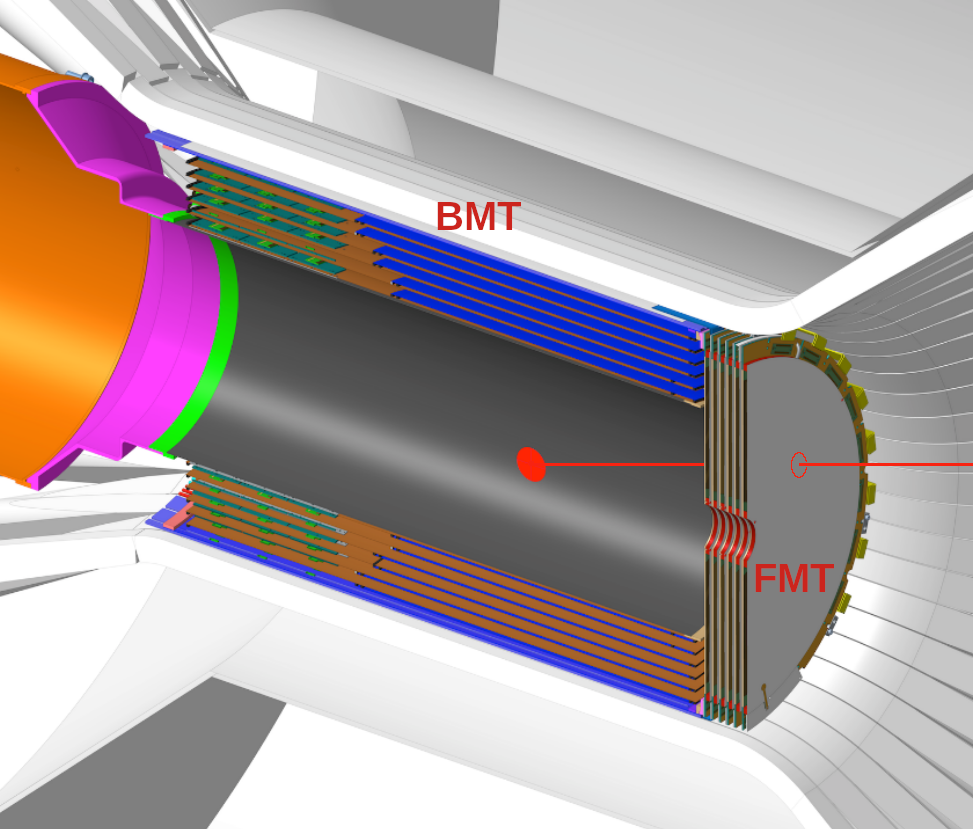
\includegraphics[scale=0.5]{10mvt.png}}
        \caption[MVT detector.]{MVT detector.
        The red dot denotes the $z=0$ point in the beamline, the red line denotes an arbitrary track coming from that point, and the circumference in the Forward MicroMegas Tracker (FMT) denotes where that track produces a signal in an FMT layer.
        Source: \hyperlink{jlab.org/physics/hall-b/clas12}{CLAS12 wiki}.}
        \label{fig::12.10::micromegas_vertex_tracker}
    \end{figure}

    Similar to the division of CLAS12 into a central detector and a forward detector, the MVT is also divided into two parts to maximise the angular coverage.

    The first component is the Barrel MicroMegas Tracker (BMT), which consists of 18 cylindrical detectors arranged in 6 layers.
    When combined with the SVT, this detector covers the angular region from $35$ to $125$ degrees, significantly enhancing the resolution of the polar angle \cite{acker2020mvt}.

% --+ FMT +---------------------------------------------------------------------
    Then, the Forwards MicroMegas Tracker (FMT), which is made of six circular, flat detectors covering angles from $6$ to $29\degree$.
    In theory, it should improve the vertex resolution by a factor of $3$ to $10$ when compared to the Drift Chambers (DC) \cite{aune2009}.
    While the original design of the FMT included six layers, the current implemented detector has only three layers installed.
    This is due to technical difficulties and concerns regarding its Lorentz angle \cite{konczykowski2010}.

    Each of the three FMT layers has $1024$ readout strips, which follow a peculiar distribution, as can be seen in the image to the right of Figure \ref{fig::12.10::fmt_geometry}.
    In addition, each layer's orientation differs by $60\degree$ to provide an accurate measurement in the xy-plane, as is shown in the image at the centre of the same Figure \cite{acker2020mvt}.

    \begin{wrapfigure}{r}{0.50\textwidth}
        \centering\frame{
        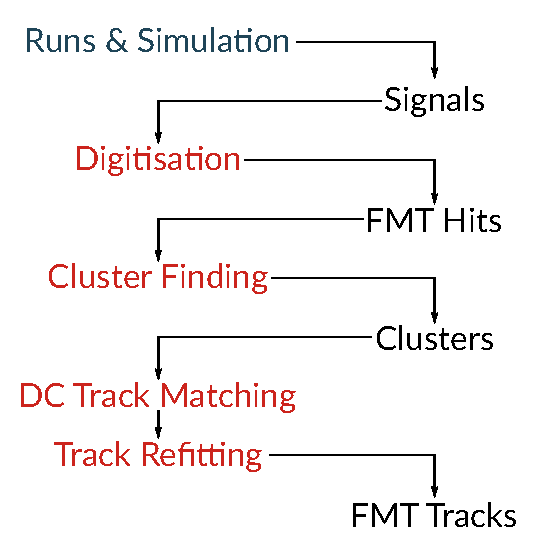
\includegraphics[width=\linewidth]{10fmt_recon.pdf}}
        \caption[FMT reconstruction summary]{FMT reconstruction summary.
        Data taking is coloured blue, data in black, and processes in red.
        Source: Own elaboration using \hyperlink{inkscape.org/}{Inkscape}.}
        \label{fig::12.11::fmt_reconstruction}
    \end{wrapfigure}

    The FMT is composed of six circular, flat detectors that cover angles ranging from $6$ to $29$ degrees.
    In its conception, it was anticipated that the FMT would improve the vertex resolution by a factor of 3 to 10 compared to the DC \cite{aune2009}.
    However, the currently implemented FMT deviates from the original design, with only three layers installed.
    This modification was necessitated by technical difficulties and concerns related to its Lorentz angle \cite{konczykowski2010}.

    Each of the three FMT layers is equipped with 1024 readout strips that exhibit a distinctive distribution, as depicted in the image on the right-hand side of Figure \ref{fig::12.10::fmt_geometry}.
    Additionally, the orientation of each layer differs by 60 degrees to ensure accurate measurements in the xy-plane, as illustrated in the image at the center of the same Figure \cite{acker2020mvt}.

    \begin{figure}[t]
        \centering\frame{
        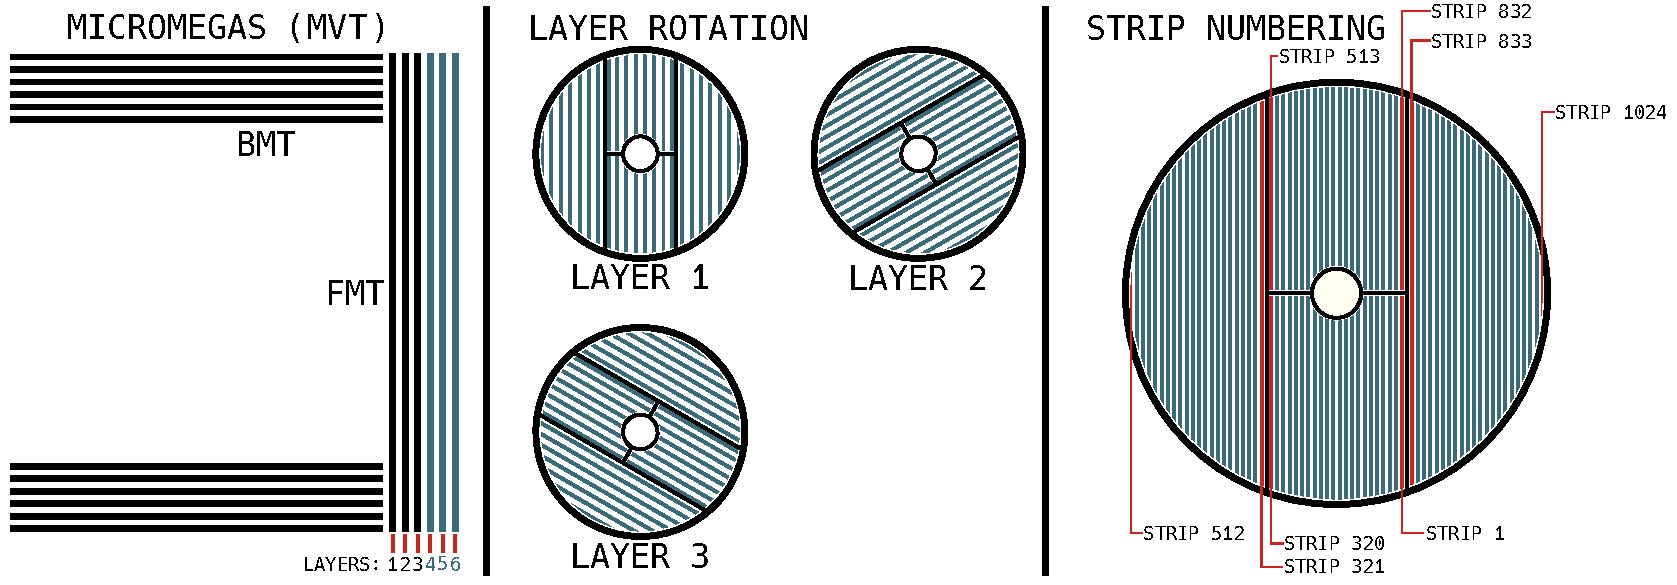
\includegraphics[width=\textwidth]{10fmt_geometry.pdf}}
        \caption[FMT detector geometry.]{FMT detector geometry. The first picture shows the distribution of the BMT and FMT layers, the second the different angle of each FMT layer, and the third the readout strip distribution of each FMT layer.
        Source: Own elaboration, using \hyperlink{inkscape.org/}{Inkscape}.}
        \label{fig::12.10::fmt_geometry}
    \end{figure}

    % !TEX root = ../main.tex
\subsubsection{FMT Track Reconstruction}
\label{sssec::fmt_track_reconstruction}
    Once a signal is detected on a readout strip and the data is stored, the information is extracted from it during offline reconstruction.
    The reconstruction process of the FMT closely resembles that of the DC.

    To begin with, when a signal is detected in a strip, it undergoes digitisation, processing, and is transformed into an \textbf{FMT Hit}.
    A set of FMT hits is then processed using a \textbf{Cluster Finding} algorithm, where a \textbf{Cluster} is defined as a group of hits that likely originate from the same particle track.
    Groups of clusters from different layers are subjected to a \textbf{DC Track Matching} algorithm, where they are matched to DC tracks generated by the DC Reconstruction process.
    Subsequently, a \textbf{Track Refitting} algorithm is employed for each DC track using the data from the clusters, resulting in updated tracks known as \textbf{FMT tracks}.
    An overview of this entire process is provided in Figure \ref{fig::fmt_recon}.


    % !TEX root = ../main.tex
\subsection{FMT Alignment}
\label{ssec::fmt_alignment}
% --+ Why is it needed +--------------------------------------------------------
    While in a perfect world the target and each detector would be installed precisely where they are needed, in the real world there is an unavoidable misalignment in their positions.
    This misalignment needs to be addressed and included into reconstruction:
    the software needs to be aware of where a detector is positioned in relation to the target to provide meaningful results.

    In the CLAS collaboration, the Calibration and Commissioning group (CalCom) is in charge of the alignment and calibration of each detector.
    Shifts and rotations that need to be applied for alignment are included in the Calibration and Conditions Database (CCDB), which is then read in reconstruction. % NOTE. A citation would be cool.

    The main goals of alignment work were three:
    First, to provide FMT alignment tables to Run Group F (RG-F) so that they may be used in reconstruction.
    Second, to check if the resolution improvement from FMT is good enough to justify the extra material added to the CLAS12 detector.
    Finally, to provide detailed information about these improvements so that Run Group E (RG-E) and other run groups can choose if they will include the detector to their runs.

% --+ Definitions +-------------------------------------------------------------
    Alignment shifts can be made in any of the three global axes:
    $z$, which is concentric to the beamline, $x$, which is parallel to the ground, and $y$, which points up from the ground.
    Then, alignment rotations can be done in any of these axes, and for the purposes of this work will be referred to as $\phi$ rotation (roll), when they're done around the $z$ axis, and pitch and yaw when they're done around the $x$ and $y$ axes respectively.

    To measure misalignment, we define a the Distance Of Closest Approach (DOCA) between a reconstructed DC track and an FMT cluster as a \textbf{Residual}.
    Due to each layer's geometry (refer to figure \ref{fig::fmt_geometry}), only the residuals in a layer's local $y$ axis (perpendicular to the strips) can be measured.
    This means that global $z$ and $\phi$ alignment can be done for each layer independently, but global $x$, global $y$, pitch, and yaw alignment has to be done for the entire detector at once.

% --+ How was it done +---------------------------------------------------------
    \begin{figure}[b!]
        \centering\frame{
        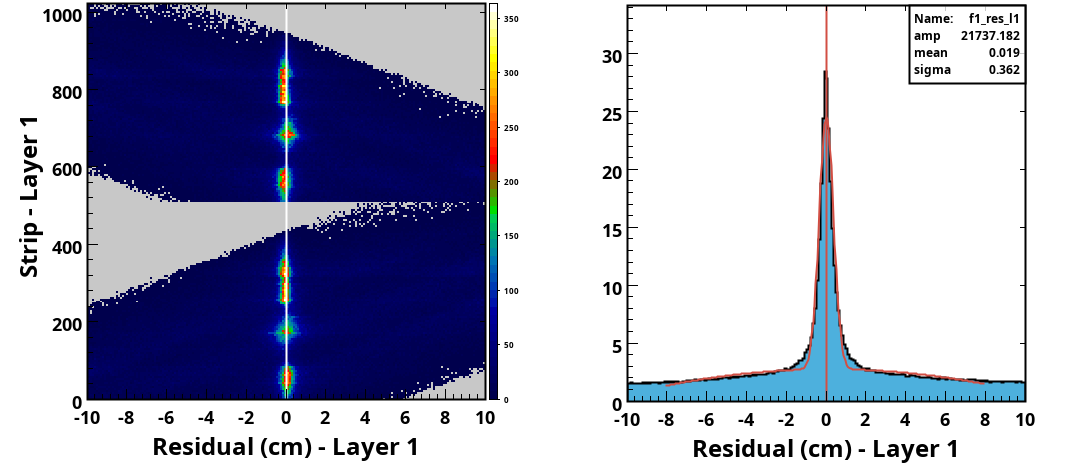
\includegraphics[width=\textwidth]{20res_example.png}}
        \caption[Example FMT residuals plot]{Example FMT residuals plot.
        Source: \hyperlink{github.com/JeffersonLab/clas12alignment}{CLAS12 alignment software}.}
        \label{fig::res_example}
    \end{figure}

    To minimise residuals, they are plotted for a particular shift or rotation in any of the relevant axes.
    An example of such a plot is shown in figure \ref{fig::res_example}.
    Since a Gaussian distribution is to be expected for the residuals, a Gaussian fit is applied to them.
    For $z$ and $\phi$ alignment, the goodness of a fit is evaluated heuristically by comparing their $\sigma$ and choosing the shift with the minimum $\sigma$.
    Then, for $x$, $y$, pitch, and yaw alignment, the goodness of a fit is evaluated heuristically by choosing the fit with the mean closest to $0$.
    The minimums are of course chosen within a healthy error margin.
    Examples of $z$ and $xy$ goodness of fit distributions can be seen in figure \ref{fig::resfit_example}.

    \begin{figure}[t!]
        \centering\frame{
        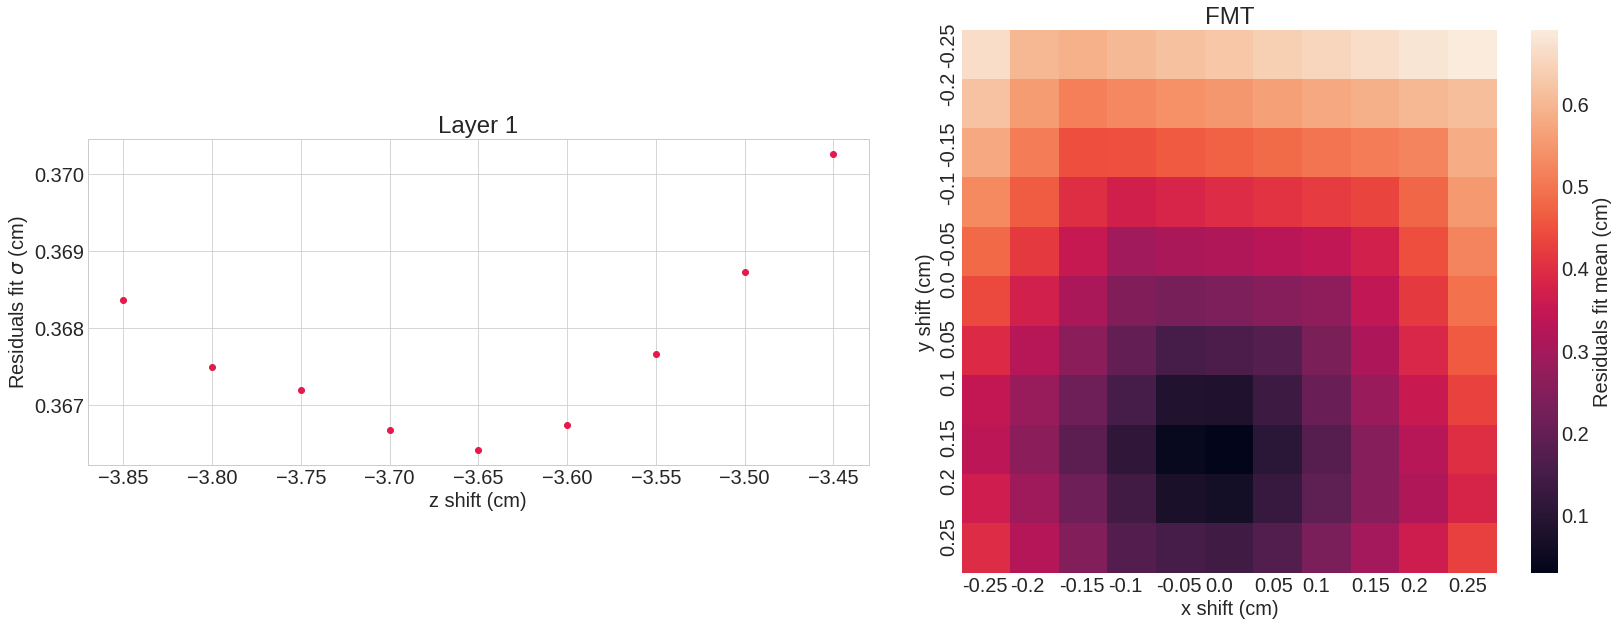
\includegraphics[width=\textwidth]{20resfit_example.png}}
        \caption[Examples of residuals goodness of fit plots]{Examples of residuals goodness of fit plots.
        Source: \hyperlink{github.com/JeffersonLab/clas12alignment}{CLAS12 alignment software}.}
        \label{fig::resfit_example}
    \end{figure}

% --+ Cuts +--------------------------------------------------------------------
\subsubsection{Fiducial Cuts}
    To reduce background, fiducial cuts are applied to the DC tracks and FMT clusters.
    This process is useful to increase data quality in order to obtain meaningful alignment results.

    For DC tracks, the cuts applied are:
    \begin{itemize}
        \item $\text{track}.z < \text{layer}.z$:
        Remove tracks with a vertex $z$ further downstream than the FMT layer before swimming.
        This is caused by reconstruction errors where the particle origin is outside of the target.
        % $9.84\%$ of tracks fail to meet this criterion in the sample data.
        \item $\mid\text{track}.z - \text{layer}.z\mid < 0.05 \text{cm}$:
        Remove tracks too far from the FMT layer after swimming.
        This was caused by bugs in the swimmer which will be mentioned in the next section.
        % $18.67\%$ tracks failed to meet this criterion.
        \item $5 \text{cm} < \sqrt{x^2 + y^2} < 25 \text{cm}$:
        Remove tracks outside of the layer's active region.
        % $35.22\%$ of the tracks were lost to this criterion.
        \item $\theta < ~66.42^{\circ}$:
        Remove tracks with a $\theta$ angle too high.
        When this happens, the same particle is affecting many strips, which causes the detector's data to not be as reliable as we want for alignment.
        % $7.22\%$ of tracks were lost to this criterion.
    \end{itemize}
    % From all these criteria, $70.95\%$ of the DC tracks were lost.
    % It is worth noting that after some reconstruction errors were fixed (as will be detailed in the following section), this percentage was reduced to $52.28\%$.

    For FMT clusters, the cuts applied are:
    \begin{itemize}
        \item $50 \text{ns} < \text{T}_{\text{min}} < 500 \text{ns}$:
        Cut clusters with an illogical $\text{T}_{\text{min}}$, which is the time of the first hit in the cluster.
        % $21.12\%$ of clusters fail to meet this criterion.
        \item $\text{size} > 1$ $\&\&$ $\text{E} > 100$:
        Cut small clusters with high energy, which are generally considered bad.
        % Only $7.36\%$ clusters are lost to this criterion.
        \item $\text{size} < 5$:
        Cut large clusters, which are not considered very useful.
        % Only $7.77\%$ are lost to this criterion.
    \end{itemize}
    % From all these criteria, $36.25\%$ of the FMT clusters were lost.

% --+ Minimisation of residuals +-----------------------------------------------
\subsubsection{Residuals Improvements}
    To validate the alignment algorithm proposed, it was tested on RG-F data (run $\mathbf{11983}$).
    The improvement in residuals is immediately obvious, as can be seen in figure \ref{fig::res_comparison}, noting the difference in scale between the top and bottom plots.

    \begin{figure}[t!]
        \centering\frame{
        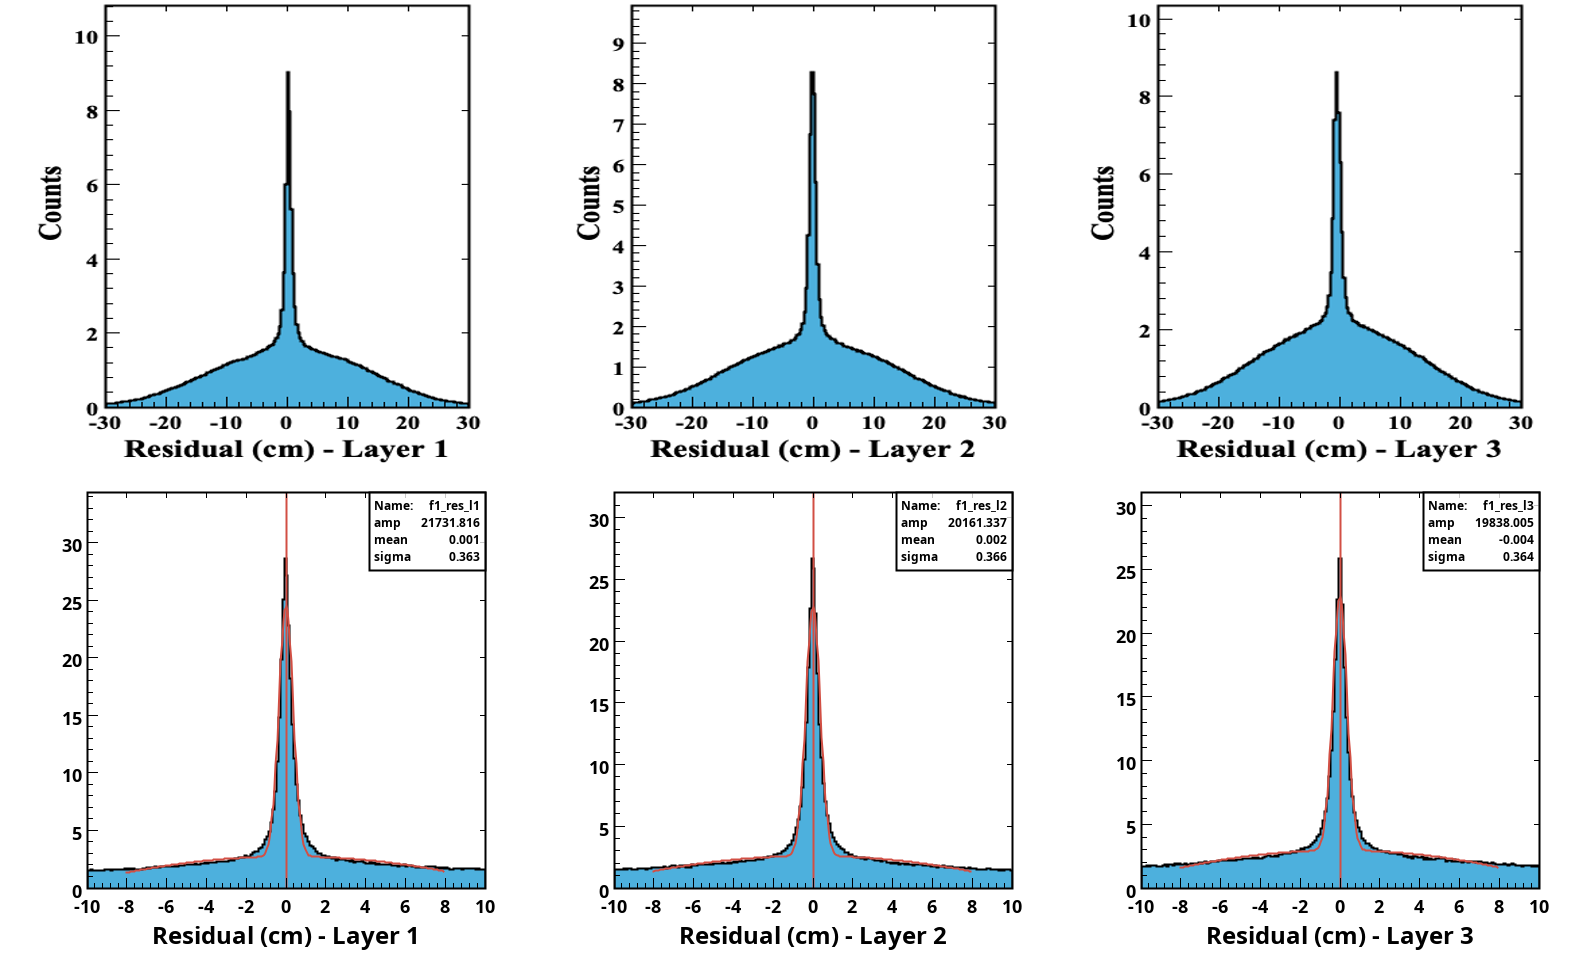
\includegraphics[width=\textwidth]{20res_comparison.png}}
        \caption[Residuals distribution improvement.]{Residuals distribution before (upper image) and after (lower image) alignment.
        Source: \hyperlink{github.com/JeffersonLab/clas12alignment}{CLAS12 alignment software}.}
        \label{fig::res_comparison}
    \end{figure}

    As can be seen in the figure, the $z$ and $\phi$ alignment heavily reduces the background, increasing the number of residuals near the mean of the distribution.
    In addition, the $x$ and $y$ alignment pushes this mean to zero, whereas it was slightly off before.
    Finally, no meaningful results were obtained for pitch and yaw alignment.
    This is attributed to how small the rotations around the $x$ and $y$ axes are, compounded with the fact that three layers do not provide enough data to perform alignment precise enough.

    To measure the mean and $\sigma$ of the distribution, a Gaussian fit was used.
    Its parameters are

     \begin{align*}
        \Big( \text{amp} \cdot \text{gaus}(\mu, \sigma) \Big) &+ \Big( p_0 + p_1\cdot x + p_2\cdot x^2 \Big) \\
        \text{gaussian} \hspace{0.8cm} &+ \hspace{1cm} \text{background}
    \end{align*}

    The results obtained are included in the CCDB at:

    \small\href{clasweb.jlab.org/cgi-bin/ccdb/versions?table=/geometry/fmt/alignment}{\texttt{clasweb.jlab.org/cgi-bin/ccdb/versions?table=/geometry/fmt/alignment}}

    Alignment was also later performed for Run Group M (RG-M) data successfully, proving that the alignment procedure is agnostic to a particular run.
    How this alignment procedure affects the resolution of the entire CLAS12 detector will be explored at the end of the chapter.

    The procedure described in this section is documented and shared publicly.
    It can be seen at:

    \href{github.com/JeffersonLab/clas12alignment/tree/master/fmt}{\texttt{github.com/JeffersonLab/clas12alignment/tree/master/fmt}}

    % !TEX root = ../main.tex
\subsection{FMT Reconstruction Work}
\label{ssec::fmt_reconstruction_work}
% --+ Why is it needed +--------------------------------------------------------
    As the work on FMT alignment progressed, certain modifications were required in FMT reconstruction.
    These modifications primarily involved incorporating the alignment shifts determined during the alignment process into the reconstruction.
    Additionally, some fixes were made to address issues that were identified during the alignment work.
    These changes ensure that the reconstruction process takes into account the alignment information and addresses any related issues that were encountered.

% --+ What was done +-----------------------------------------------------------
    First, the loading of shifts from the CCDB was included in the standard geometry class of the FMT reconstruction package.
    Then, standard methods to include the shifts in any frame of reference change were implemented.
    Finally, the code was studied in detail, and the shifts were added in all instances where they were required since the package originally didn't consider their application.

    ``Crossmaking'' is the process of matching clusters in different layers to obtain an accurate 3D estimate of the position of a track \cite{ziegler2020}.
    This process was initially included in FMT reconstruction to facilitate the reconstruction for the six FMT layers.
    However, as mentioned before, only three FMT layers were installed for the RG-F run, and future runs may also use three layers due to concerns with the Lorentz angle when using six layers.
    To simplify the reconstruction process and make better use of the available number of layers, crossmaking was removed from the reconstruction.

    Outside of FMT reconstruction, some minor changes were also required in the DC reconstruction package since some of its components depend on the FMT layers' positions.
    Additionally, the swim package diagnostic was updated as it failed to properly reconstruct the positions of tracks near the FMT layers.

% --+ Juicy link +--------------------------------------------------------------
    A detailed list of the updates applied can be found in the following pull request to the \texttt{clas12-offline-software} repository:

    \href{github.com/JeffersonLab/clas12-offline-software/pull/726}{\texttt{github.com/JeffersonLab/clas12-offline-software/pull/726}}.

    % !TEX root = ../main.tex
\subsection{Validation and Results}
\label{12.40::validation_and_results}
% --+ Data used +---------------------------------------------------------------
    Just like the residuals validation, the results presented in this document are based on the application of this work to RG-F data.
    It is important to note that the RG-F target is approximately 55 centimetres long, which is much larger than the average CLAS12 target \cite{hattawy2019}.
    Specifically, the runs used for testing and validation are presented in Table \ref{tab::12.40::rgf_data}, and the run used to obtain the data displayed in this section was 011983.

    \begin{table}[h!]
        \centering
        \begin{tabular}{lllll}
            \toprule
            \textbf{Run Number} & \textbf{Energy (MeV)} & \textbf{Current (nA)} & \textbf{Configuration} & \textbf{Target} \\
            \midrule \midrule
            011983              & 10389.4               &  50                   & Inbending              & D2 \\
            012016              & 10389.4               & 250                   & Inbending              & D2 \\
            012439              &  2186.4               &  15                   & Inbending              & H2 \\
            012461              & 10196.6               &  20                   & Inbending              & D2 \\
            \bottomrule
        \end{tabular}

        \caption{RG-F runs used for validation.}
        \label{tab::12.40::rgf_data}
    \end{table}

    % !TEX root = ../main.tex
\subsubsection{Cuts}
\label{12.41::cuts}
    \begin{figure}[b!]
        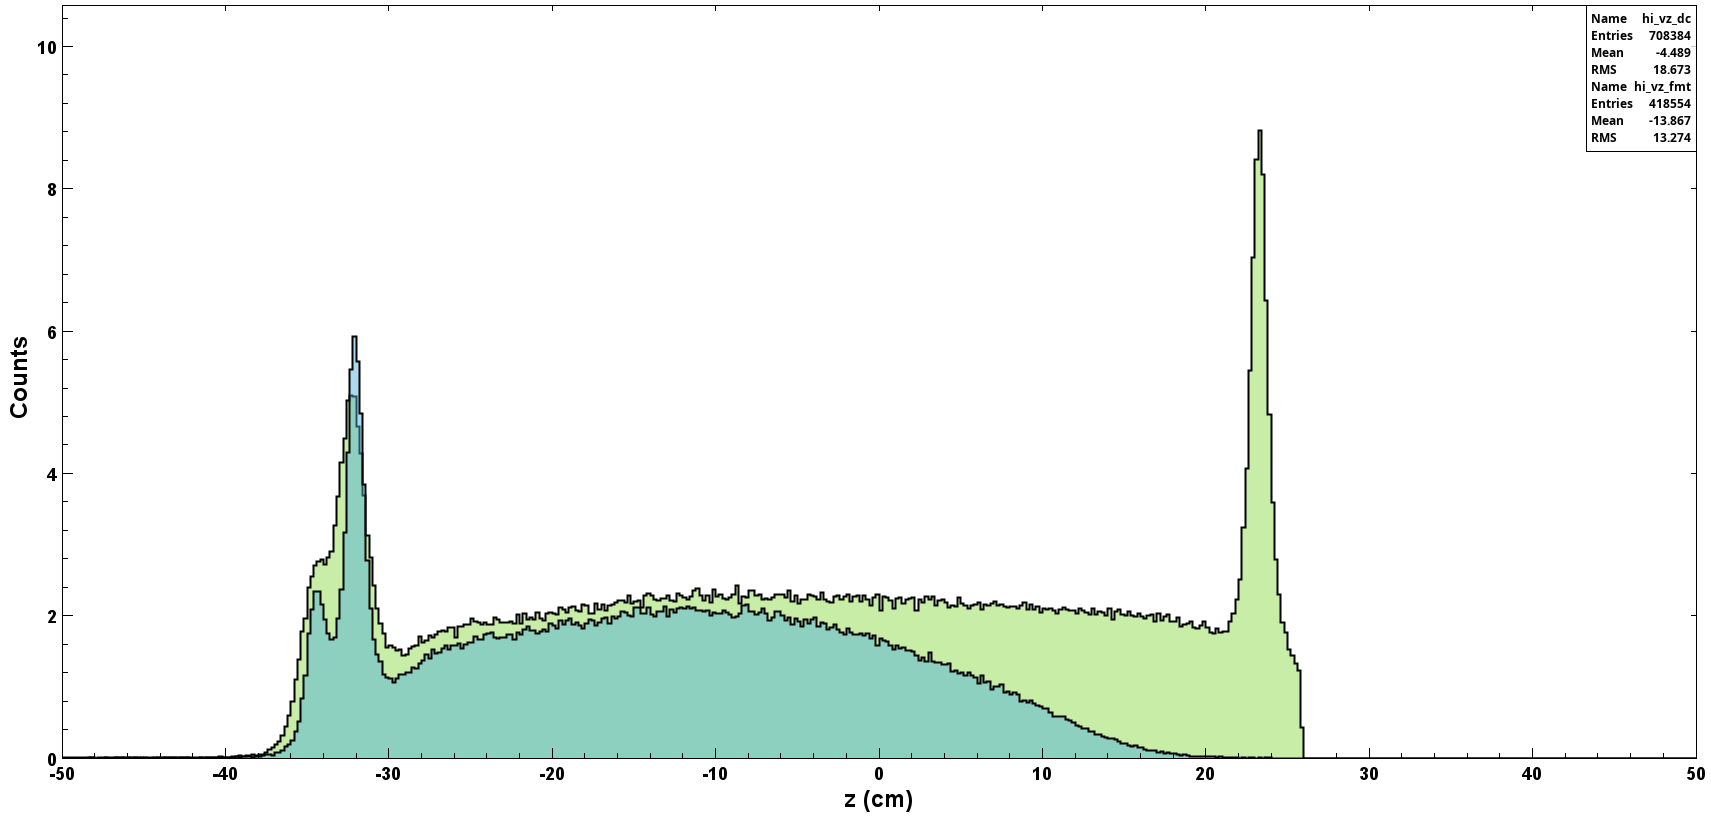
\includegraphics[width=\textwidth]{41dc_vs_fmt.png}
        \caption[DC vs. FMT $z$ without geometric correction]
        {DC vs. FMT vertex $z$ for electrons without any geometric correction.
        DC tracks are shown in green while FMT tracks are shown in blue.
        Note that the dark cyan colour comes from the overlap.}
        \floatfoot{Source: Own elaboration, using the \texttt{fmtVertex.groovy} script in \href{https://github.com/JeffersonLab/clas12alignment}{CLAS12 alignment software}.}
        \label{fig::12.41::dc_vs_fmt_vz_11983}
    \end{figure}

    Some additional cuts are applied to the tracks to obtain the plots presented in this section.
    These cuts are used to remove very poor tracks that would not be suitable for analysis regardless.
    The applied cuts are as follows:
    \begin{itemize}
        \item
            \texttt{abs(chi2pid) < 5}:
            This cut removes tracks that do not provide sufficient certainty regarding the particle's PID.
        \item
            \texttt{vz < fmtZ}:
            This cut removes tracks located further downstream than the FMT.
        \item
            \texttt{chi2/ndf < 15}:
            This cut excludes tracks with excessively high uncertainty.
    \end{itemize}

    % !TEX root = ../main.tex
\subsubsection{Geometry Effect}
\label{12.42::geometry_effect}
    To evaluate the enhancement in vertex resolution, we will compare the vertex positions of tracks that underwent only DC reconstruction with those that underwent both DC and FMT reconstruction.
    For convenience, we will refer to the former as DC tracks and the latter as FMT tracks.
    Considering that the $z$ axis is aligned with the beamline, Figure \ref{fig::12.41::dc_vs_fmt_vz_11983} illustrates the $z$ positions of the vertex for DC tracks versus FMT tracks.

    To comprehend the plot in Figure \ref{fig::12.41::dc_vs_fmt_vz_11983}, it is valuable to examine the RG-F target.
    The target consists of a large gas-filled chamber with a varying composition across different runs.
    The distance between the chamber windows measures $553.32$ millimetres.
    Furthermore, it was observed that the upstream window of the target is positioned approximately $24$ millimetres away from the beam window.
    All windows are constructed from aluminium and have a thickness of $15$ micrometers.
    A detailed depiction of the target can be found in Addendum 1.

    Based on Figure \ref{fig::12.41::dc_vs_fmt_vz_11983}, it is evident that the FMT detector solely detects the upstream windows, completely overlooking the downstream one.
    This issue stems from a geometric constraint: the downstream window falls outside the active detection area of the FMT.
    This effect is clearly illustrated in Figure \ref{eq::12.42::vz_vs_theta}, where the $\theta$ angle is plotted against the vertex $z$ coordinate.
    The two red lines in the plots represent the FMT's active area, and it is apparent that the downstream window lies outside this region, thereby explaining its absence.

    \begin{figure}[t!]
        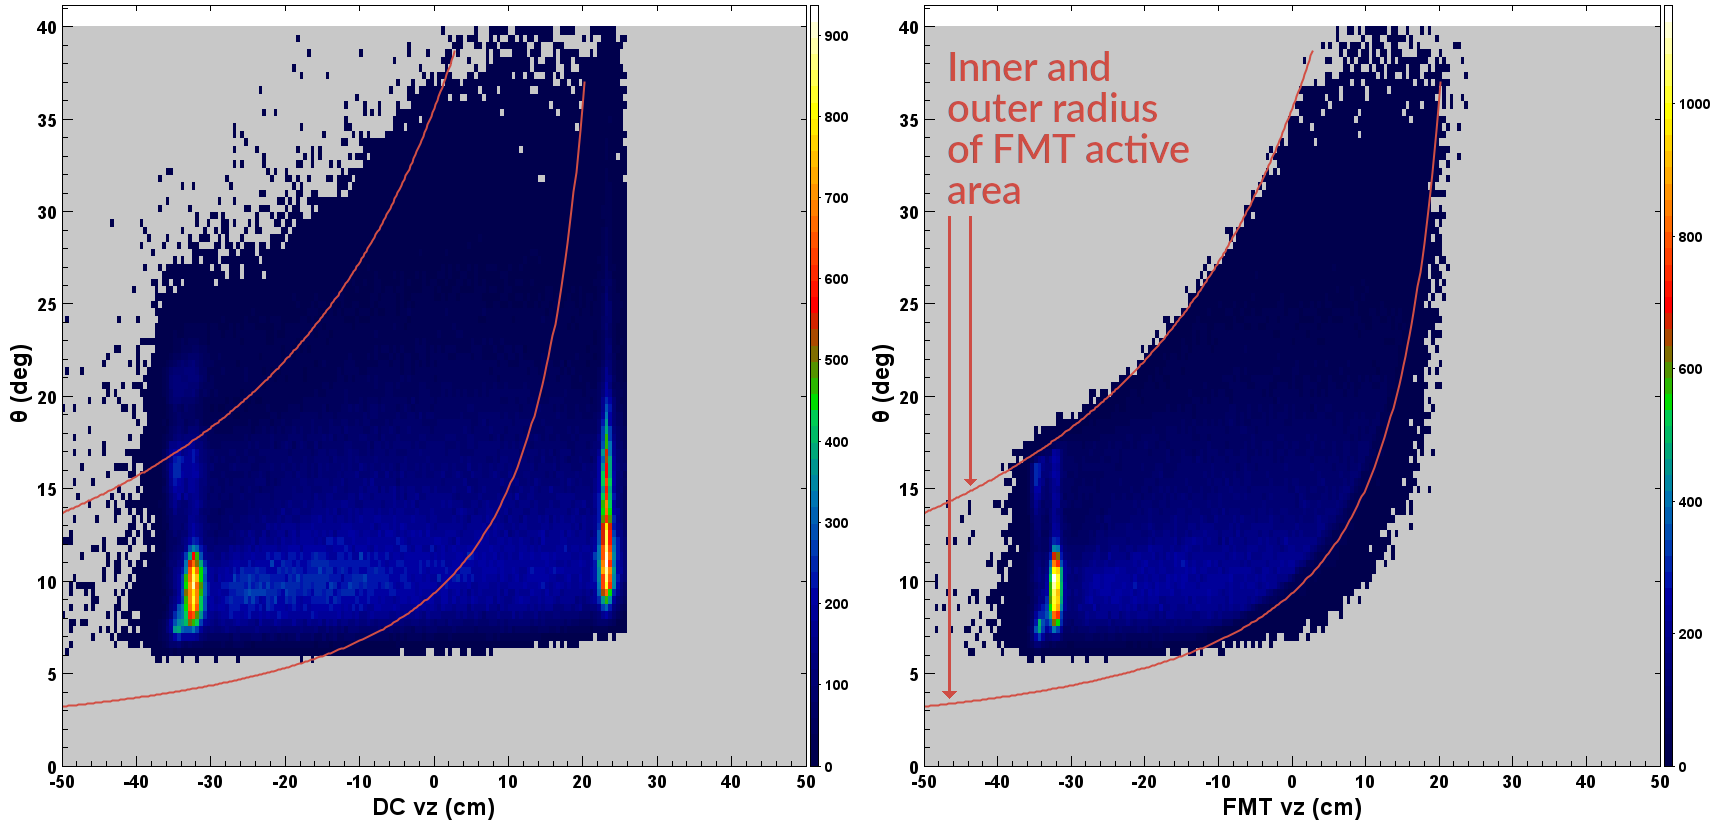
\includegraphics[scale=0.24]{42theta_dc_vs_fmt.png}
        \caption[$z$ vs. $\theta$ for DC and FMT]
        {$z$ vs. $\theta$ for DC and FMT for electrons without any geometry correction.
        FMT's active area are shown in red lines.}
        \floatfoot{Source: Own elaboration, using the \texttt{fmtVertex.groovy} script in \href{https://github.com/JeffersonLab/clas12alignment}{CLAS12 alignment software}.}
        \label{eq::12.42::vz_vs_theta}
    \end{figure}

    To compensate for this geometric effect, we introduce an additional cut based on the plotted curves.
    The curves can be described by the following equations
    \begin{equation}
        c_1(z) = 57.29 \cdot \arctan\left(\frac{r_\text{inner}}{z_0 - z}\right),
        \hspace{0.5cm}
        c_2(z) = 57.29 \cdot \arctan\left(\frac{r_\text{outer}}{z_0 - z}\right).
        \label{eq::12.42::fmt_geometry_cut}
    \end{equation}

    Here, $r_\text{inner}$ represents the radius of the hole at the center of the FMT, $r_\text{outer}$ denotes the radius of the outer circumference of the FMT, and $z_0$ corresponds to the $z$ position of the first FMT layer plus the drift distance.
    All these parameters are obtained from the CCDB.

    % !TEX root = ../main.tex
\subsubsection{Vertex Resolution Improvement}
\label{12.43::vertex_resolution_improvement}

    \begin{figure}[b!]
        \frame{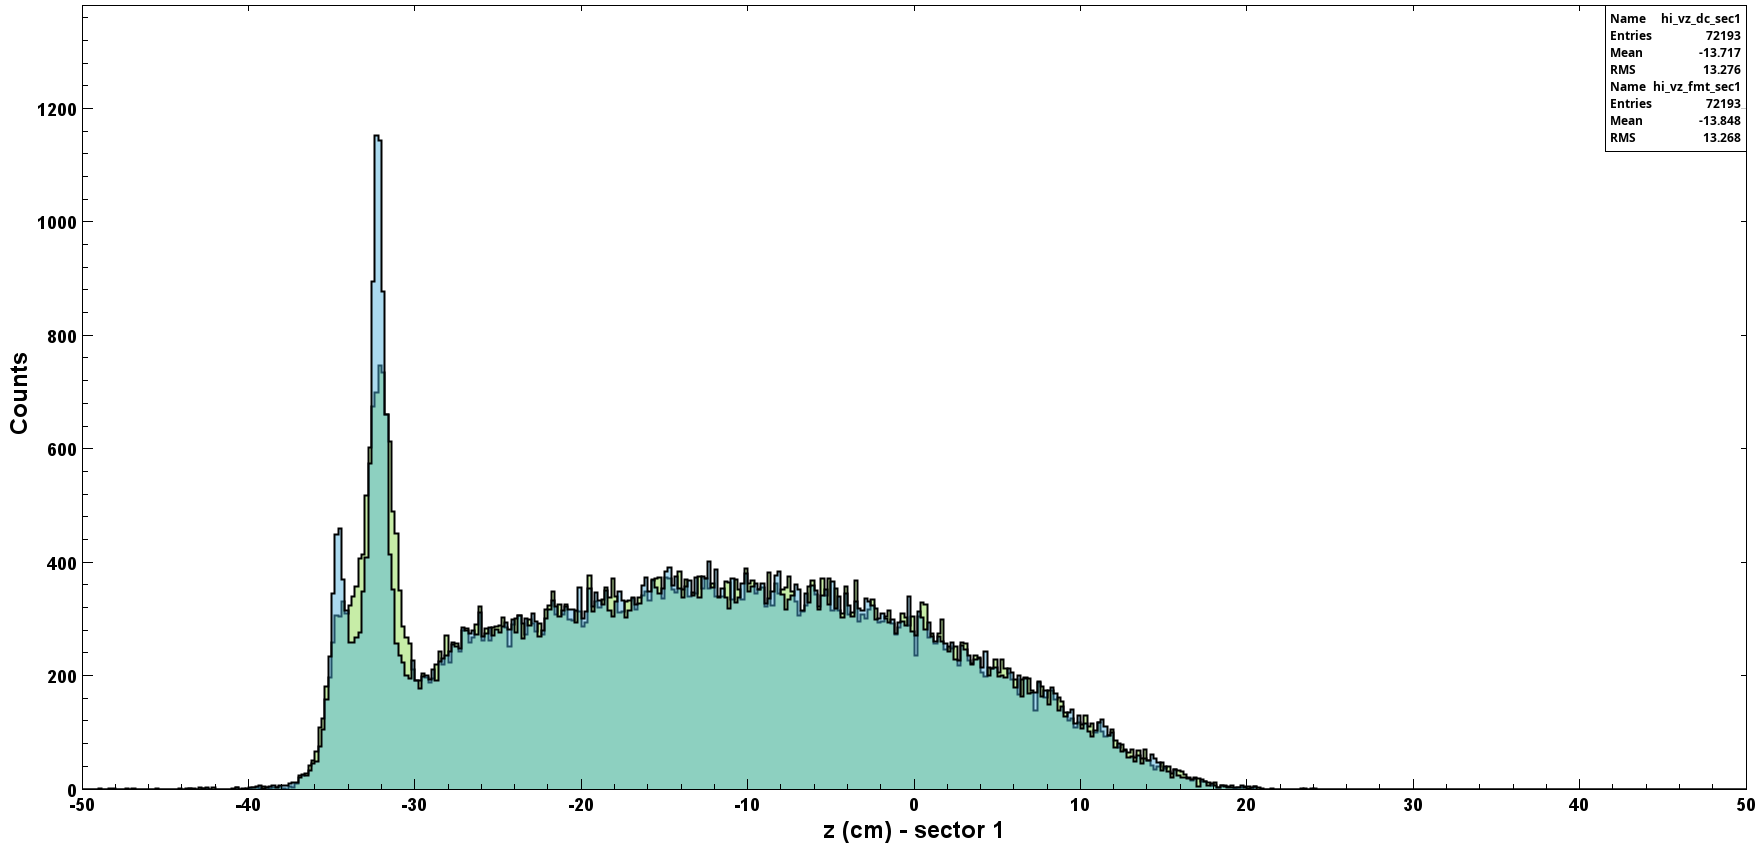
\includegraphics[scale=0.24]{40dc_vs_fmt_sector1.png}}
        \caption[DC vs FMT $z$ with geometry correction]
        {DC vs FMT vertex $z$ for electrons with a geometric correction.
        DC tracks are shown in green while FMT tracks are shown in blue.
        Data from only one CLAS12 sector was used to obtain this plot.}
        \floatfoot{Source: Own elaboration, using the \texttt{fmtVertex.groovy} script in \href{https://github.com/JeffersonLab/clas12alignment}{CLAS12 alignment software}.}
        \label{fig::12.43::dc_vs_fmt_vz_11983_corrected}
    \end{figure}

    Furthermore, an additional cut has been introduced.
    As of the FMT alignment work, beam alignment for RG-F data had not been carried out, resulting in a decrease in vertex resolution.
    To mitigate the impact of this alignment issue on reconstruction accuracy, we have implemented a cut to utilise only one sector of the detector.

    The resolution plot, comparing DC and FMT tracks after applying all the previously mentioned cuts, is depicted in Figure \ref{fig::12.43::dc_vs_fmt_vz_11983_corrected}.
    To evaluate the resolution for both DC and FMT tracks, we utilise a fit consisting of two Gaussian curves combined with a quadratic curve to account for the background.
    The fit is defined as follows
    \begin{equation*}
        \text{amp}_1 \cdot \text{gaus}(z, z_\text{max}, \sigma) + \text{amp}_2 \cdot \text{gaus}(z, z_\text{max} - 2.4, \sigma) + p_1 + p_2\cdot z + p_3\cdot z^2,
    \end{equation*}
    where
    \begin{itemize}
        \item
            $\text{amp}1$ represents the amplitude of the largest peak, and $z\text{max}$ corresponds to its $z$ position,
        \item
            $\text{amp}_2$ signifies the amplitude of the leftward peak, which has been measured to be at a position of $2.4$ centimetres, and
        \item
            the remaining parameters, $p_1$, $p_2$, and $p_3$, are obtained through the fitting process.
    \end{itemize}

% --+ Resolution for electrons +------------------------------------------------
    For electrons in run 011983 (low luminosity, 50 nA), the analysis yields a DC resolution of $\sigma_\text{DC} = 0.875$ cm and an FMT resolution of $\sigma_\text{FMT} = 0.387$ cm.
    This indicates a doubling of the resolution achieved with the inclusion of the FMT detector.

    Similarly, for electrons in run 012016 (production luminosity, $250$ nA), the analysis shows a DC resolution of $\sigma_\text{DC} = 1.009$ cm and an FMT resolution of $\sigma_\text{FMT} = 0.596$ cm.

    % !TEX root = ../main.tex
\subsubsection{Conclusions}
\label{12.44::conclusions}
    Although the improvement in resolution is not as significant as initially anticipated for the detector, it remains an encouraging result.
    The enhanced resolution enables more precise measurements of the target position.
    As a practical implication, it allows for double targets to be positioned closer to each other, thereby benefiting the derived physics from experiments like the RG-E run.

    The reason for the smaller-than-predicted improvement in resolution can be attributed to the initial projection, which assumed the presence of six FMT layers.
    The inclusion of six layers would provide additional positional data along the particle's track, thereby enhancing the accuracy of the vertex position measurement during the fitting process.

% --+ Why no improvements is seen on vertex momentum resolution +---------------
    Furthermore, due to the limited number of layers and their close proximity in the FMT detector, it exhibits a small lever arm.
    As a result, the detector's contribution to the vertex momentum resolution is not significant, as it does not provide sufficient additional data to accurately determine the track's momentum.

% --+ Show detector efficiency +------------------------------------------------
    In order to gain a better understanding of the FMT detector, we conducted a brief study on its efficiency.
    The efficiency is defined as the ratio of the number of FMT tracks to the number of DC tracks, representing how many of the DC tracks were also detected by the FMT.

    For the three-layer configuration, the efficiency is approximately $88.96\%$.
    Figure \ref{fig::12.44::fmt_azimuthal_efficiency} illustrates the layer-by-layer efficiency, showing no anomalous geometric effects.
    The observed gaps in efficiency are solely a result of the CLAS12 detector's geometry, which is divided into six sectors.

    \begin{figure}[b]
        \centering\frame{
        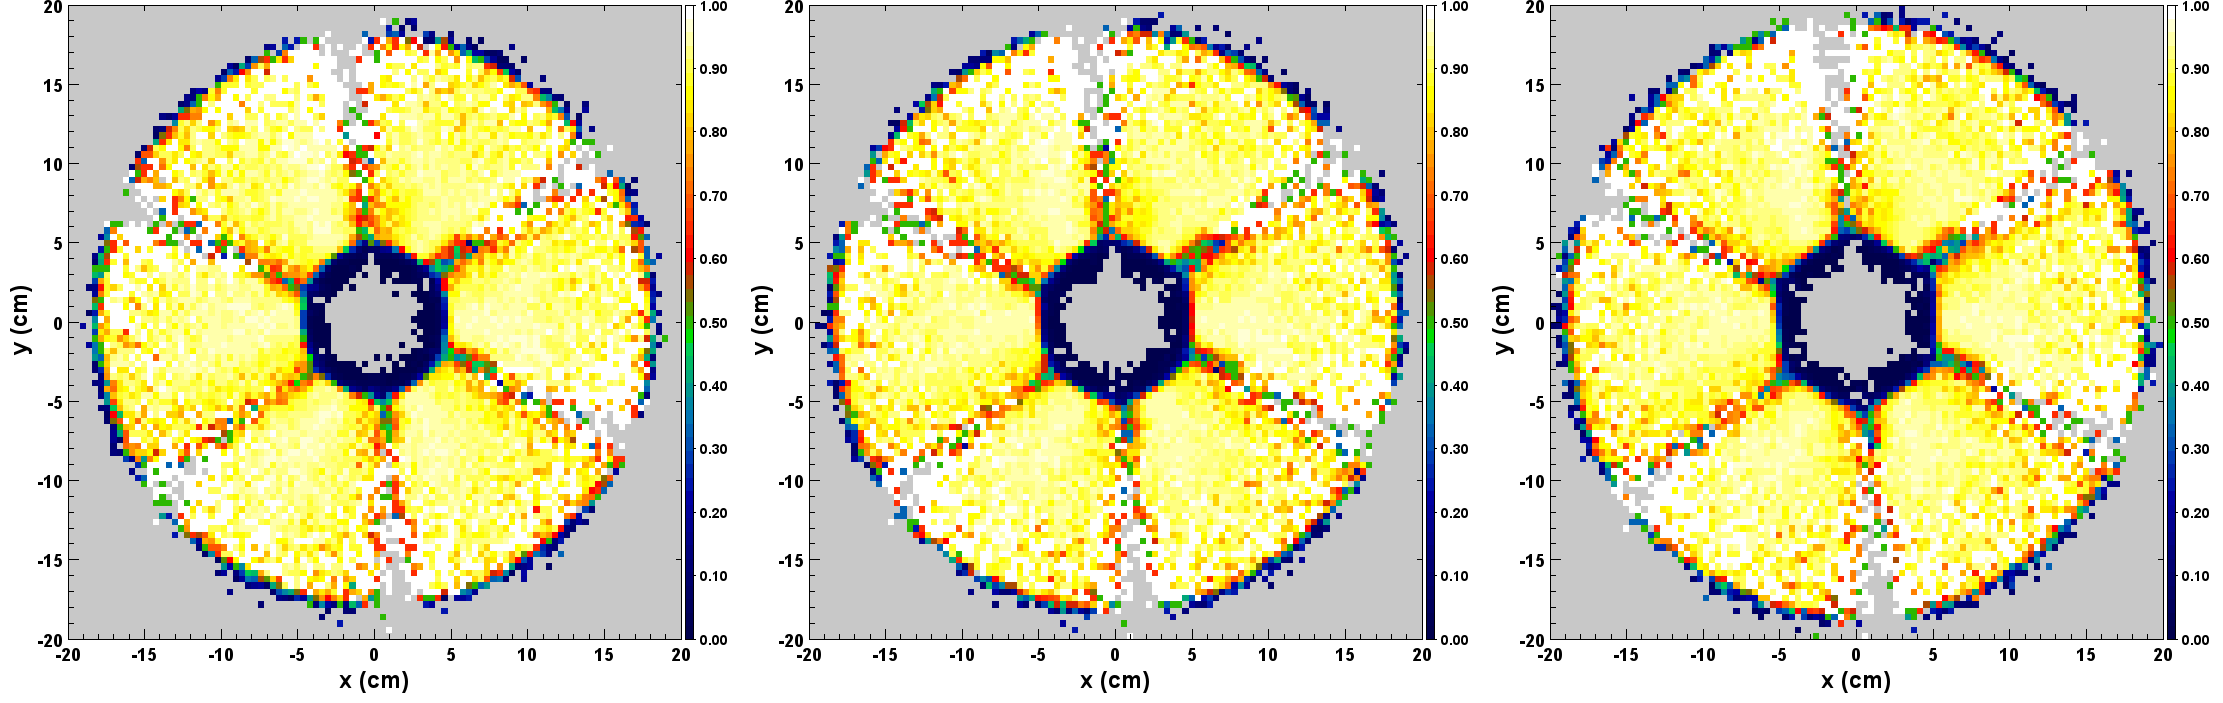
\includegraphics[width=\textwidth]{44fmt_efficiency.png}}
        \caption[FMT layers efficiency]{Efficiency of each FMT layer.
        Source: \texttt{fmtVertex.groovy} script in \hyperlink{github.com/JeffersonLab/clas12alignment}{CLAS12 alignment software}.}
        \label{fig::12.44::fmt_azimuthal_efficiency}
    \end{figure}


